\begin{frame}
	\frametitle{Disconnect, Privacy Badger (EFF), Ghostery}

	\begin{center}
		
\includegraphics[height=0.7\textheight]{../../img/disconnectme.jpg}
	\end{center}
\end{frame}
\note{Auf dem PC und Laptop ist das vorgehen gegen Tracking leicht. Es gibt Addons für Chrome, Firefox etc. die Webseiten die Kommunikation mit Trackern einfach verbieten. Disconnect und Privacy Badger sind dabei Open Source und sollten wenn möglich dem bekannteren Ghostery vorgezogen werden.}

\begin{frame}
	\frametitle{Antitracking im Firefox Privatmodus}

	\begin{center}
		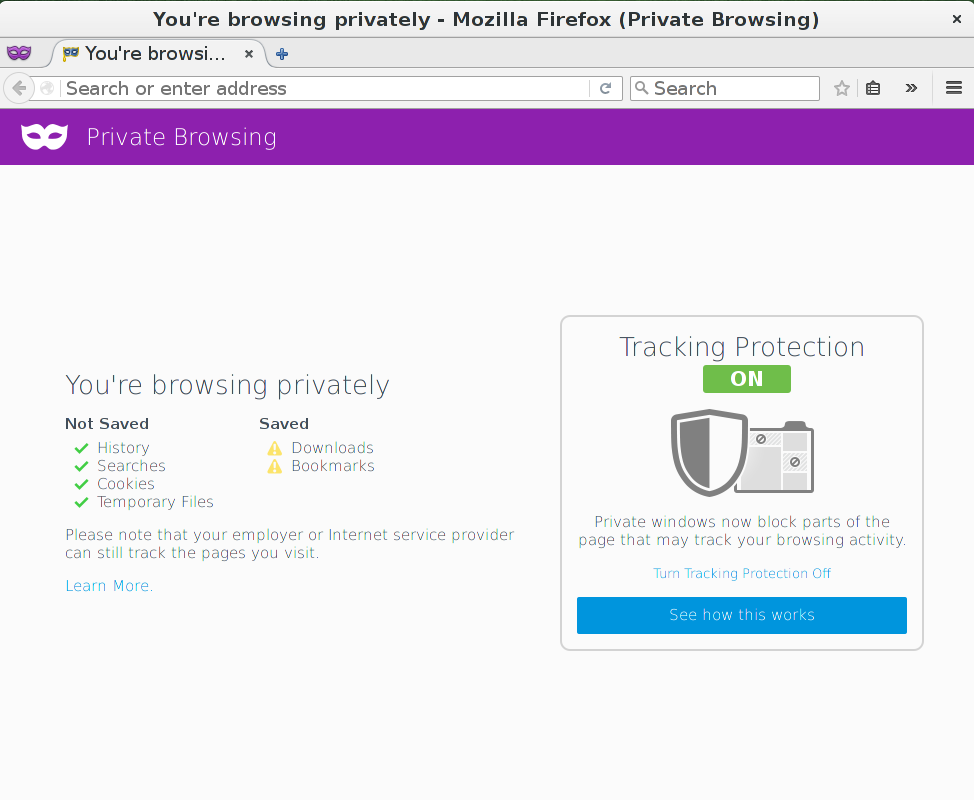
\includegraphics[height=0.7\textheight]{../../img/ff_antitrack.png}
	\end{center}
\end{frame}
\note{Auch der Privatmodus im Firefox kann mittlerweile Tracking verbieten. Er benutzt dafür die Sperrliste von Disconnect. Aber eines der Addons nutzen ist trotzdem besser weil das dann auch im normalen Modus funktioniert. Alternativ kann man als Firefox-Benutzer auch das Addon ``Enable Tracking Protection'' benutzen, dann ist der eingebaute Trackingschutz immer aktiv.}

\begin{frame}{Antitracking auf dem Handy}
	\begin{columns}
		\column{5.5cm}
		\footnotesize
		\textbf{Firefox auf Android}\\
		Firefox-Menü -> Extras -> Addons -> Alle Firefox-Addons ansehen -> nach Tracking suchen -> Addon "Enable Tracking Protection" installieren.

		\textbf{Android: Google AdID}\\
		Google-Einstellungen -> Anzeigen -> Interessensbezogene Werbung deaktivieren\\
		\vspace{0.5cm}

		\textbf{iOS: Apple IDFA}\\
		Einstellungen -> Datenschutz -> Werbung -> Kein Ad-Tracking\\
		\vspace{0.5cm}

		\column{5cm}

		\begin{center}
			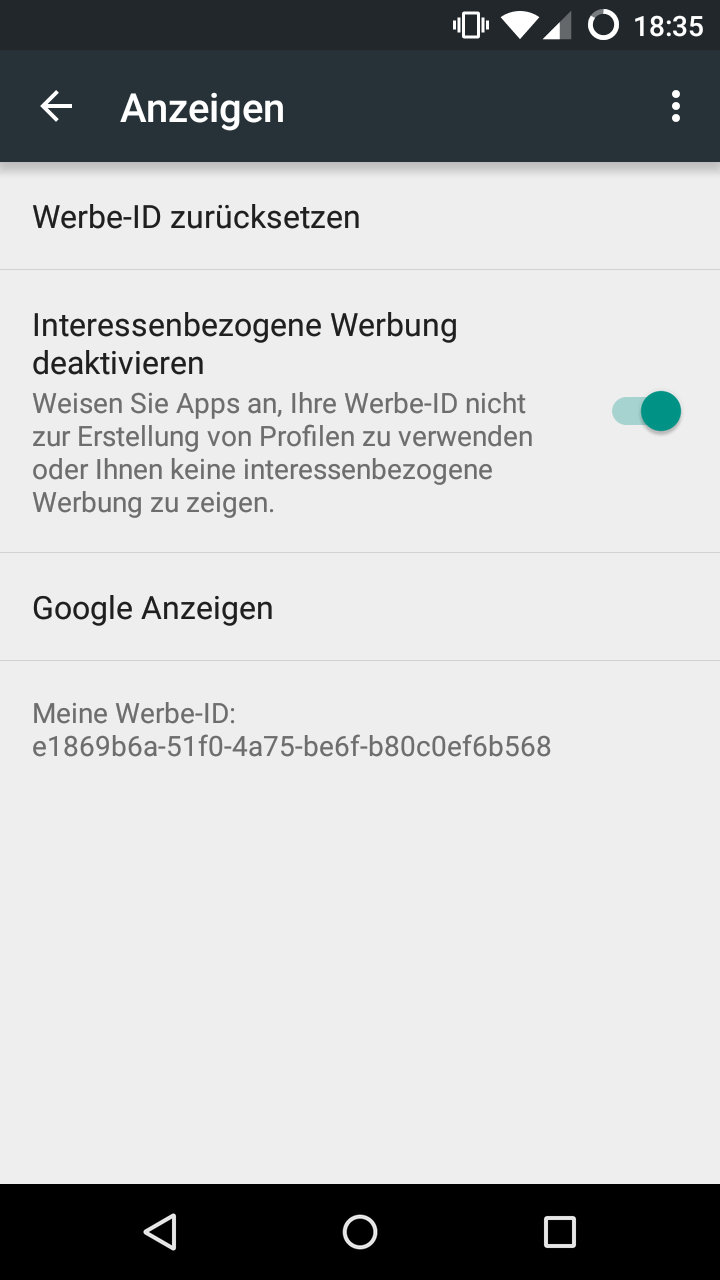
\includegraphics[width=3.5cm]{../../img/google-adid.png}
		\par\end{center}
	\end{columns}
\end{frame}
\note{Auf dem Handy gibt es leider nur eine uns bekannte Möglichkeit: ein Firefox-Addon auf Android. Immerhin sieht es bei Apps besser aus, da kann man das Tracking verbieten und zwar global für alle. Das liegt daran, dass auf iOS und Android den Apps das Tracken nur mit einer von Apple oder Google für jeden Nutzer vergebenen, eindeutigen ID erlaubt ist. Diese kann man wie auf der Folie gezeigt deaktivieren.}
